\begin{definition}
    This is the first definition of the first homework.
\end{definition}
\begin{exercise}[label=ex:H.1.1]
    This is the first exercise of the first homework.
\end{exercise}
\begin{proof}
    This is the first proof of the first exercise of the first homework. We can easily reference labels from \codeinline{text}{main.tex}, e.g. \zcref{thm:1.1}.
\end{proof}

\begin{exercise}[label=ex:H.1.2]
    This is the second exercise of the first homework.
\end{exercise}
\begin{proof}
    This is the first proof of the second exercise of the first homework. We reference \zcref{ex:H.1.1} here.
\end{proof}

\begin{exercise}[label=ex:H.1.3]
    This is the third exercise of the first homework.
\end{exercise}
\begin{answer}
    The answer to \zcref{ex:H.1.3}
\end{answer}

We insert \zcref{fig:Three_Plane_Orthogonal_Complements} as an example figure:
\begin{figure}[H]
    \centering
    \includegraphics[page=2]{Three_Planes_Orthogonal_Complements_licensed_under_CC_BY-SA_4.0.pdf}
    \caption{A figure whose author \extref{https://github.com/GrassGlass}{Grass} licenses under \extref{https://creativecommons.org/licenses/by-sa/4.0/}{CC BY-SA 4.0}.}
    \label{fig:Three_Plane_Orthogonal_Complements}
\end{figure}